\documentclass[aspectratio=169]{beamer}
\usecolortheme{dove}
\usepackage{hyperref}
\usepackage{url}
\usepackage{cite}
\usepackage{tikz}
\usepackage{graphicx}
\usepackage{xcolor}
\definecolor{mycolor}{rgb}{0.0, 0.44, 1.0} 
\hypersetup{
    colorlinks=true,       
    linkcolor=mycolor,       
    citecolor=mycolor,          
    urlcolor=mycolor          
}
\definecolor{maroon}{rgb}{0.65, 0.16, 0.16}
\setbeamersize{text margin left=1.5em}  % <- remove for 4:3 aspect ratios 
\setbeamersize{text margin right=1.5em} % <- remove for 4:3 aspect ratios
\setbeamertemplate{frametitle}{\vspace{10pt} \color{maroon} \insertframetitle}
\usepackage{multirow}
\usepackage{makecell}
\usepackage{ragged2e}

\defbeamertemplate*{footline}{mytheme}
    {
       \leavevmode%
       \hbox{%
       \begin{beamercolorbox}[wd=.5\paperwidth,ht=2.25ex,dp=1ex,center]{author in head/foot}%
         \usebeamerfont{author in head/foot}\insertshortauthor~~(\insertshortinstitute)
       \end{beamercolorbox}%
       \begin{beamercolorbox}[wd=.5\paperwidth,ht=2.25ex,dp=1ex,right]{title in head/foot}%
         \usebeamerfont{title in head/foot}\insertshorttitle{}\hspace*{2em}
         \insertframenumber{} / \inserttotalframenumber\hspace*{2ex} 
       \end{beamercolorbox}}%
       \vskip0pt%
    }
    \usebeamertemplate{mytheme}
\setbeamercolor*{item}{fg=maroon}
\setbeamertemplate{itemize items}[triangle] 
\setbeamertemplate{itemize subitem}[square] 
\setbeamertemplate{itemize subsubitem}[circle] 


%--------------------------------------------------
% Title
%--------------------------------------------------

\title{\color{maroon} Multiple OLS Regression}
\subtitle{\textit{\color{maroon} IBEI Teaching Fellowship Example}}
\author{\href{https://alhdzsz.netlify.com/}{Alfredo Hernandez Sanchez, Ph.D.}}
\institute{\href{https://www.ibei.org/en}{Barcelona Institute of International Studies}} 
\date{\today}


%--------------------------------------------------
% Custom
%--------------------------------------------------
\usebackgroundtemplate{
	\tikz[overlay,remember picture] 
	\node[opacity=0.6, at=(current page.north east),anchor=north east,inner sep=0pt] {
    
\includegraphics[height= 9cm]{background}};
  }
  
\usepackage{caption}
\captionsetup{labelformat=empty}
\usepackage{tcolorbox}

%--------------------------------------------------
\begin{document}
%--------------------------------------------------
\maketitle

%--------------------------------------------------
\begin{frame}
\frametitle{Question and Hypothesis}

\begin{tcolorbox}[colframe=maroon,title=Example Code]
The MTCARS dataset is included within R and is commonly used as an example for graphs and learning new packages. You can follow these examples by consulting the \href{https://github.com/alhdzsz/IBEI-Example/blob/master/cars_script.R}{script} on GitHub. 
\end{tcolorbox}
\Large
\vspace{.5cm}
\begin{itemize}
    \item What increases the fuel economy of a car?
    \begin{itemize}
        \item H1: Lighter cars (kg) are more fuel efficient (km/liter).
    \end{itemize}
\end{itemize}


\end{frame}


%--------------------------------------------------
\begin{frame}
\frametitle{Ordinary Least Squares}

\begin{center}
    Multiple Regression Model
\end{center}
\Large
\begin{equation}
y = \beta_{0} + \beta_{1}x_{1} + \beta_{2}x_{2} + ... + \beta_{p}x_{p} + \epsilon
\end{equation}

\vspace{.5cm}
\normalsize
\noindent Where $y$ is the dependent variable, \\
$x_{1:p}$ are the independent variables, \\  
$\beta_{0:p}$ are the coefficients, \\
and $\epsilon$ is the error (residual)

\end{frame}

%--------------------------------------------------
\begin{frame}
\frametitle{Selecting Independent Variables}

\begin{columns}

\column{0.5\textwidth}
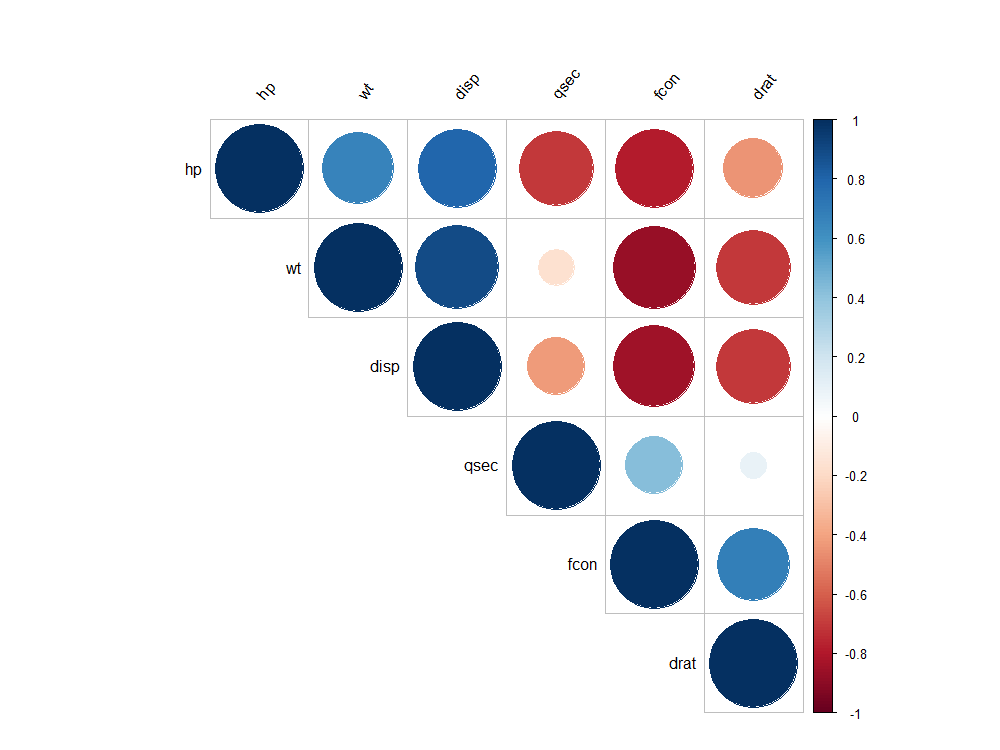
\includegraphics[height=.8\textheight]{correlogram}


\column{0.5\textwidth}
\scriptsize
\begin{table}[]
\begin{tabular}{lllllll}
     & fcon  & hp    & wt    & qsec  & disp  & drat  \\
fcon & 1     & -0.78 & -0.87 & 0.42  & -0.85 & 0.68  \\
hp   & -0.78 & 1     & 0.66  & -0.71 & 0.79  & -0.45 \\
wt   & -0.87 & 0.66  & 1     & -0.17 & 0.89  & -0.71 \\
qsec & 0.42  & -0.71 & -0.17 & 1     & -0.43 & 0.09  \\
disp & -0.85 & 0.79  & 0.89  & -0.43 & 1     & -0.71 \\
drat & 0.68  & -0.45 & -0.71 & 0.09  & -0.71 & 1    
\end{tabular}
\end{table}

\end{columns}

\end{frame}

%--------------------------------------------------
\begin{frame}
\frametitle{Variables}

\begin{columns}

\scriptsize
\column{0.4\textwidth}
\begin{itemize}
\item	fcon:	Km./Liter
\item	cyl:	Number of cylinders
\item	disp:	Displacement (cu.in.)
\item	hp:	Gross horsepower
\item	drat:	Rear axle ratio
\item	wt:	Weight (tons)
\item	qsec:	1/4 mile time
\item	vs:	Engine (0 = V-shaped, 1 = straight)
\item	am:	Transmission (0 = automatic, 1 = manual)
\item	gear:	Number of forward gears
\item	carb:	Number of carburetors
\end{itemize}

\column{0.6\textwidth}

\tiny
\begin{table}[!htbp] \centering 
  \caption{Descriptive statistics} 
  \label{} 
\begin{tabular}{@{\extracolsep{5pt}}lccccccc} 
\\[-1.8ex]\hline 
\hline \\[-1.8ex] 
Statistic & \multicolumn{1}{c}{N} & \multicolumn{1}{c}{Mean} & \multicolumn{1}{c}{St. Dev.} & \multicolumn{1}{c}{Min} & \multicolumn{1}{c}{Pctl(25)} & \multicolumn{1}{c}{Pctl(75)} & \multicolumn{1}{c}{Max} \\ 
\hline \\[-1.8ex] 
mpg & 32 & 20.1 & 6.0 & 10 & 15.4 & 22.8 & 34 \\ 
disp & 32 & 230.7 & 123.9 & 71 & 120.8 & 326 & 472 \\ 
hp & 32 & 146.7 & 68.6 & 52 & 96.5 & 180 & 335 \\ 
drat & 32 & 3.6 & 0.5 & 2.8 & 3.1 & 3.9 & 4.9 \\ 
wt & 32 & 1.5 & 0.4 & 0.7 & 1.2 & 1.6 & 2.5 \\ 
qsec & 32 & 17.8 & 1.8 & 14.5 & 16.9 & 18.9 & 22.9 \\ 
vs & 32 & 0.4 & 0.5 & 0 & 0 & 1 & 1 \\ 
gear & 32 & 3.7 & 0.7 & 3 & 3 & 4 & 5 \\ 
carb & 32 & 2.8 & 1.6 & 1 & 2 & 4 & 8 \\ 
fcon & 32 & 8.5 & 2.6 & 4.4 & 6.6 & 9.7 & 14.4 \\ 
\hline \\[-1.8ex] 
\end{tabular} 
\end{table} 

\end{columns}
\end{frame}

%--------------------------------------------------
\begin{frame}
\frametitle{Scatterplot}

\begin{center}
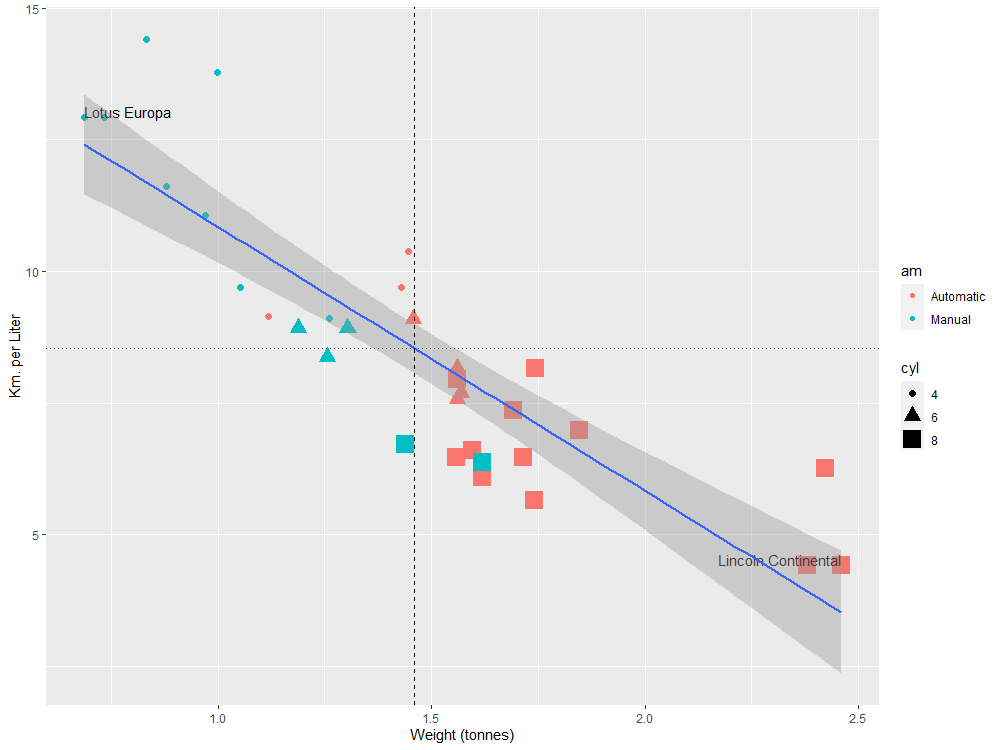
\includegraphics[height=.8\textheight]{scatterplot}
\end{center}

\end{frame}

%--------------------------------------------------
\begin{frame}

\vspace{-1cm}

\tiny

\begin{table}[!htbp] \centering 
  \caption{} 
  \label{} 
\begin{tabular}{@{\extracolsep{5pt}}lcccc} 
\\[-1.8ex]\hline 
\hline \\[-1.8ex] 
 & \multicolumn{4}{c}{\textit{Dependent variable:}} \\ 
\cline{2-5} 
\\[-1.8ex] & \multicolumn{4}{c}{Km. per Liter} \\ 
\\[-1.8ex] & (1) & (2) & (3) & (4)\\ 
\hline \\[-1.8ex] 
 Weight (kg) & $-$11.048$^{***}$ & $-$8.016$^{***}$ & $-$5.951$^{***}$ & $-$5.161$^{***}$ \\ 
  & (1.156) & (1.308) & (1.871) & (1.831) \\ 
  & & & & \\ 
 Gross horsepower &  & $-$0.014$^{***}$ & $-$0.016$^{***}$ & $-$0.014$^{**}$ \\ 
  &  & (0.004) & (0.004) & (0.006) \\ 
  & & & & \\ 
 Type of transmission (manual=1) &  &  & 0.886 & 0.769 \\ 
  &  &  & (0.585) & (0.594) \\ 
  & & & & \\ 
 Number of Cylinders &  &  &  & $-$1.289$^{**}$ \\ 
  &  &  &  & (0.598) \\ 
  & & & & \\ 
 cyl8 &  &  &  & $-$0.920 \\ 
  &  &  &  & (0.971) \\ 
  & & & & \\ 
 Constant & 15.853$^{***}$ & 15.828$^{***}$ & 14.457$^{***}$ & 14.332$^{***}$ \\ 
  & (0.798) & (0.680) & (1.124) & (1.108) \\ 
  & & & & \\ 
\hline \\[-1.8ex] 
Observations & 32 & 32 & 32 & 32 \\ 
R$^{2}$ & 0.753 & 0.827 & 0.840 & 0.866 \\ 
Adjusted R$^{2}$ & 0.745 & 0.815 & 0.823 & 0.840 \\ 
Residual Std. Error & 1.295 (df = 30) & 1.103 (df = 29) & 1.079 (df = 28) & 1.025 (df = 26) \\ 
F Statistic & 91.375$^{***}$ (df = 1; 30) & 69.211$^{***}$ (df = 2; 29) & 48.960$^{***}$ (df = 3; 28) & 33.571$^{***}$ (df = 5; 26) \\ 
\hline 
\hline \\[-1.8ex] 
\textit{Note:}  & \multicolumn{4}{r}{$^{*}$p$<$0.1; $^{**}$p$<$0.05; $^{***}$p$<$0.01} \\ 
\end{tabular} 
\end{table} 

\end{frame}


%--------------------------------------------------
\begin{frame}
\frametitle{Model (4) Interpretation}
\Large
\begin{equation}
y_{fcon} = 14.3 - 5.1x_{wt} - 0.01x_{hp} + 0.76x_{am} - 0.9x_{cyl} \end{equation} \\
\vspace{.5cm}
\normalsize

\begin{itemize}
  
  \item A one unit increase in weight (an additional ton) results in a 5 point decrease in fuel economy (km/lt), holding horsepower, transmission and number of cylinders constant. 

  \item Our model explains around 86\% of the variation in fuel economy. However, some variables (transmission) were not statistically significant!
\end{itemize}

\end{frame}

%--------------------------------------------------
\begin{frame}{}
\centering \LARGE Thank you!
\end{frame}

%--------------------------------------------------
\end{document}
%--------------------------------------------------